% Generated from the pinned prospective report. Units in panel B are Z-expectation MAE.
\begin{figure}[htbp]
\centering
\definecolor{pooled}{HTML}{677C91}
\definecolor{target}{HTML}{176C72}
\definecolor{guard}{HTML}{9E4F32}
\begin{minipage}[t]{0.49\linewidth}
\centering
\small\textbf{(a) Improvement over C0}\\[3pt]
\resizebox{\linewidth}{!}{%
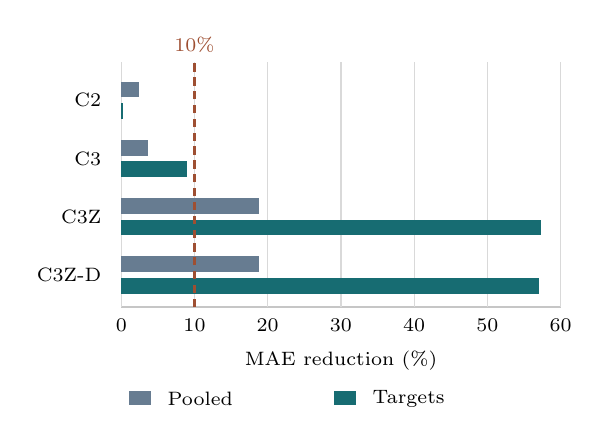
\begin{tikzpicture}[x=0.093cm,y=0.74cm,font=\scriptsize]
\draw[gray!45] (0,-.55) -- (60,-.55);
\foreach \x in {0,10,20,30,40,50,60} {
  \draw[gray!30] (\x,-.55)--(\x,3.65);
  \node[anchor=north] at (\x,-.58) {\x};
}
\node[anchor=north] at (30,-1.14) {MAE reduction (\%)};
\node[anchor=east] at (-1.4,3) {C2};
\fill[pooled] (0,3.05) rectangle (2.3558,3.32);
\fill[target] (0,2.68) rectangle (0.2616,2.95);
\node[anchor=east] at (-1.4,2) {C3};
\fill[pooled] (0,2.05) rectangle (3.6361,2.32);
\fill[target] (0,1.68) rectangle (9.0355,1.95);
\node[anchor=east] at (-1.4,1) {C3Z};
\fill[pooled] (0,1.05) rectangle (18.8431,1.32);
\fill[target] (0,0.68) rectangle (57.3676,0.95);
\node[anchor=east] at (-1.4,0) {C3Z-D};
\fill[pooled] (0,0.05) rectangle (18.8245,0.32);
\fill[target] (0,-0.32) rectangle (57.0015,-0.05);
\draw[guard,densely dashed,thick] (10,-.55)--(10,3.65);
\node[anchor=south,guard] at (10,3.65) {10\%};
\fill[pooled] (1,-2.24) rectangle (4,-2.00);
\node[anchor=west] at (5,-2.12) {Pooled};
\fill[target] (29,-2.24) rectangle (32,-2.00);
\node[anchor=west] at (33,-2.12) {Targets};
\end{tikzpicture}}
\end{minipage}\hfill
\begin{minipage}[t]{0.49\linewidth}
\centering
\small\textbf{(b) Non-target degradation (site 6)}\\[3pt]
\resizebox{\linewidth}{!}{%
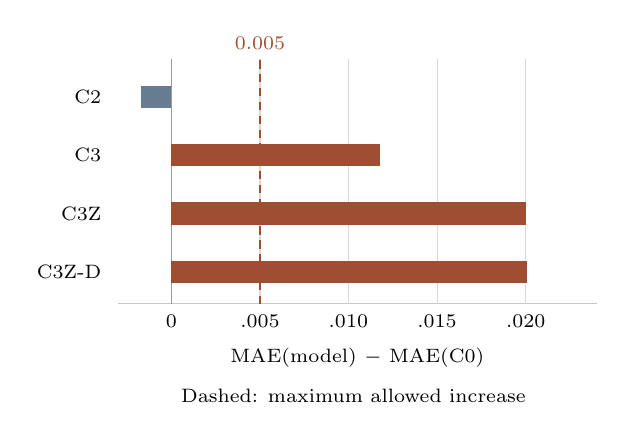
\begin{tikzpicture}[x=225cm,y=0.74cm,font=\scriptsize]
\draw[gray!45] (-.003,-.55)--(.024,-.55);
\foreach \x/\lab in {0/0,.005/.005,.01/.010,.015/.015,.02/.020} {
  \draw[gray!30] (\x,-.55)--(\x,3.65);
  \node[anchor=north] at (\x,-.58) {\lab};
}
\draw[gray!80] (0,-.55)--(0,3.65);
\node[anchor=north] at (.0105,-1.14) {MAE(model) $-$ MAE(C0)};
\node[anchor=east] at (-.0034,3) {C2};
\fill[pooled] (-0.0016914,2.81) rectangle (0.0000000,3.19);
\node[anchor=east] at (-.0034,2) {C3};
\fill[guard] (0.0000000,1.81) rectangle (0.0117888,2.19);
\node[anchor=east] at (-.0034,1) {C3Z};
\fill[guard] (0.0000000,0.81) rectangle (0.0200388,1.19);
\node[anchor=east] at (-.0034,0) {C3Z-D};
\fill[guard] (0.0000000,-0.19) rectangle (0.0200594,0.19);
\draw[guard,densely dashed,thick] (.005,-.55)--(.005,3.65);
\node[anchor=south,guard] at (.005,3.65) {0.005};
\node[anchor=west] at (0,-2.12) {Dashed: maximum allowed increase};
\end{tikzpicture}}
\end{minipage}
\caption{Frozen prospective outcomes. Panel (a) compares both registered improvement estimands with the 10\% threshold. Panel (b) shows the only non-target site that violated the degradation guardrail under C3 and its endpoint-phase extensions. Site 6 contributes six observables. All four tested candidate models fail at least one registered criterion.}
\label{fig:prospective}
\end{figure}
